\documentclass[11pt,twoside,a4paper]{scrartcl}
\usepackage[dvipsnames,svgnames]{xcolor}
\usepackage{ifpdf}
\usepackage{scrpage2}
\usepackage{footmisc}
\ifpdf
  \usepackage[pdfpagemode={UseOutlines},
              pdftitle={Model name: "S"},
              pdfauthor={Produced by SBML2LaTeX version 1.0beta},
              pdfsubject={SBML model summary},
              pdfkeywords={},
              pdfview={FitBH},
              plainpages={false},
              pdftex,
              colorlinks=true,
              pdfdisplaydoctitle=true,
              linkcolor=royalblue,
              bookmarks,
              bookmarksopen,
              bookmarksnumbered,
              pdfhighlight={/P},
              urlcolor={blue}]{hyperref}
  \usepackage{pdflscape}
  \pdfcompresslevel=9
  \usepackage[pdftex]{graphicx}
\else
  \usepackage[plainpages={false}]{hyperref}
  \usepackage{lscape}
  \usepackage{graphicx}
  \usepackage{breakurl}
\fi
\usepackage{calc}
\usepackage[paper=a4paper,landscape=false,centering]{geometry}
\usepackage{mathptmx}
\usepackage[scaled=.95]{helvet}
\usepackage[english]{babel}
\usepackage[english]{rccol}
\usepackage[version=3]{mhchem}
\usepackage{relsize}
\usepackage{pifont}
\usepackage{textcomp}
\usepackage{longtable}
\usepackage{tabularx}
\usepackage{booktabs}
\usepackage{amsmath}
\usepackage{amsfonts}
\usepackage{amssymb}
\usepackage{mathtools}
\usepackage{ulem}
\usepackage{wasysym}
\usepackage{eurosym}
\usepackage{rotating}
\usepackage{upgreek}
\usepackage{flexisym}
\usepackage{breqn}

% Introduce automatic line breaks in function calls
\makeatletter
\edef\breqn@identify@comma{\number\symletters3B}% fingers crossed!
\let\m@@Pun\m@Pun
\def\d@@Pun#1#2#3{\edef\breqn@stored@args{\number#1#2#3}
\futurelet\@let@token\d@@Punaux}
\def\d@@Punaux{%
  \expandafter\m@@Pun\breqn@stored@args
  \ifx\@let@token\@sptoken
    \ifx\breqn@stored@args\breqn@identify@comma
      \penalty\breqn@comma@penalty\relax
      \EQ@prebin@space
    \fi
  \fi
}
\def\display@setup{%
  \medmuskip\Dmedmuskip \thickmuskip\Dthickmuskip
  \let\m@Bin\d@@Bin \let\m@Rel\d@@Rel
  \let\m@Pun\d@@Pun %% new for punctuation
  \let\@symRel\d@@symRel \let\@symBin\d@@symBin
  \let\m@DeL\d@@DeL \let\m@DeR\d@@DeR \let\m@DeB\d@@DeB
  \let\m@DeA\d@@DeA
  \let\@symDeL\d@@symDeL \let\@symDeR\d@@symDeR
  \let\@symDeB\d@@symDeB \let\@symDeA\d@@symDeA
  \let\left\eq@left \let\right\eq@right \global\lr@level\z@
  \global\eq@wdCond\z@          %BRM: new
  \everyhbox{\everyhbox\@emptytoks
    \let\display@setup\relax \textmath@setup \let\textmath@setup\relax
  }%
  \everyvbox{\everyvbox\@emptytoks
    \let\display@setup\relax \textmath@setup \let\textmath@setup\relax
  }%
}
\define@key{breqn}{comma-penalty}{\def\breqn@comma@penalty{#1}}
\setkeys{breqn}{comma-penalty=5000}% break is the default
\makeatother
% End line break definition

\definecolor{royalblue}{cmyk}{.93, .79, 0, 0}
\definecolor{lightgray}{gray}{0.95}
\addtokomafont{sectioning}{\color{royalblue}}
\pagestyle{scrheadings}
\newcommand{\yes}{\parbox[c]{1.3em}{\Large\Square\hspace{-.65em}\ding{51}}}
\newcommand{\no}{\parbox[c]{1.3em}{\Large\Square\hspace{-.62em}--}}
\newcommand{\numero}{N\hspace{-0.075em}\raisebox{0.25em}{\relsize{-2}\b{o}}}
\newcommand{\reaction}[1]{\begin{equation}\ce{#1}\end{equation}}
\newcolumntype{C}[1]{>{\centering\arraybackslash}p{#1}}
\newcommand{\SBMLLaTeX}{{\sffamily\upshape\raisebox{-.35ex}{S\hspace{-.425ex}BML}\hspace{-0.5ex}\begin{rotate}{-17.5}\raisebox{-.1ex}{2}\end{rotate}\hspace{1ex}\LaTeX}}
\cfoot{\textcolor{gray}{Produced by \SBMLLaTeX}}

\subject{SBML Model Report}
\title{Model name: ``S"}
\date{\today}
\author{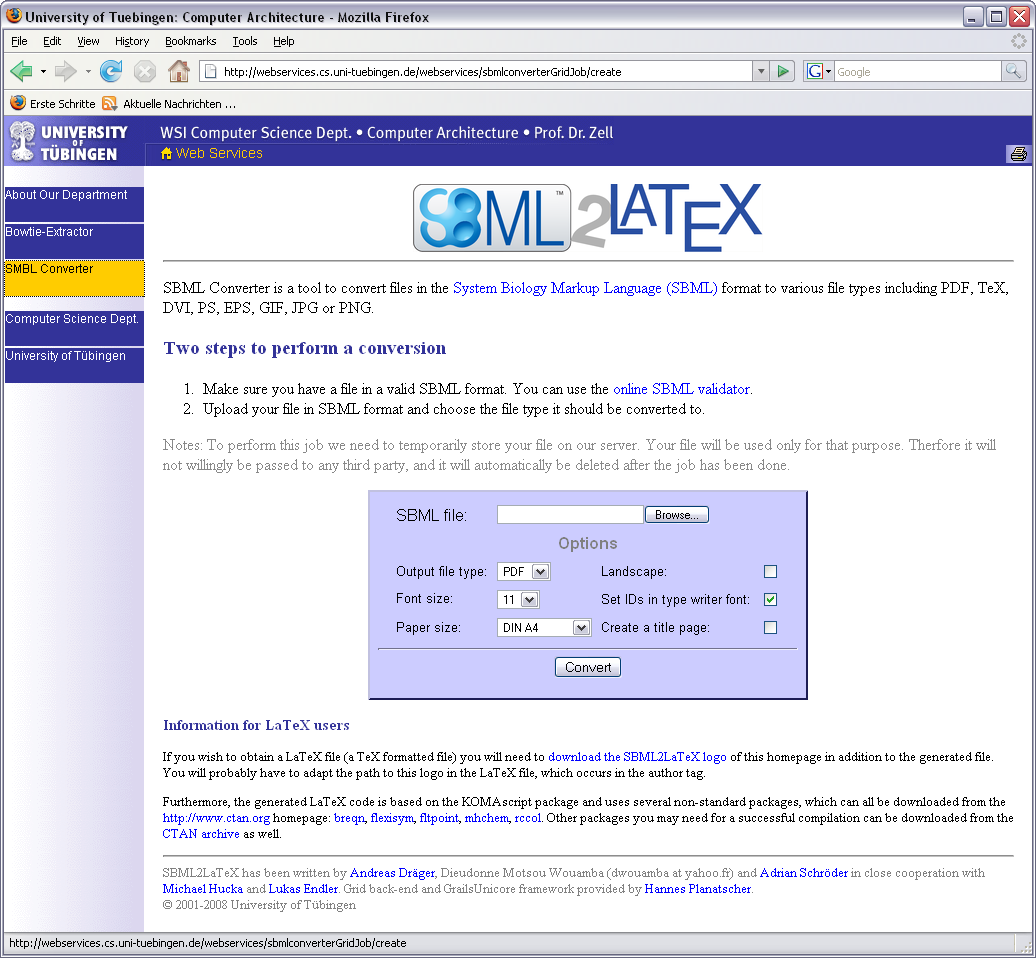
\includegraphics[height=3.5ex]{/local/draeger/workspace/DisplaySBML/resources/SBML2LaTeX}}

\begin{document}
\maketitle
\thispagestyle{scrheadings}


\section{General Overview}
This is a document in SBML Level 2 Version 3 format. Table~\ref{tab:components} shows an overview of the quantities of all components of this model.
\begin{table}[h!]
\centering
\caption{The SBML components in this model.}\label{tab:components}
All components are described in more detail in the following sections.
\begin{tabular}{l|r||l|r}
\toprule
\multicolumn{1}{c}{Element}&\multicolumn{1}{|c||}{Quantity}&\multicolumn{1}{c|}{Element}&\multicolumn{1}{c}{Quantity}\\

\midrule
compartment types&0&compartments&1\\
species types&0&species&6\\
events&0&constraints&0\\
reactions&1&function definitions&1\\
global parameters&0&unit definitions&3\\
rules&0&initial assignments&0\\
\bottomrule\end{tabular}
\end{table}

\subsection*{Model Notes}


This model has been created with the help of the SABIO-RK Database(http://sabio.villa-bosch.de/SABIORK)



\section{Unit Definitions}
This is an overview of eight unit definitions.
The units \texttt{substance}, \texttt{volume}, \texttt{area}, \texttt{length}, and \texttt{time} are predefined by SBML and not mentioned in the model.
\subsection{Unit \texttt{onedivsec}}
\begin{description}
\item[Name] onedivsec
\item[Definition] $\mathrm{s}^{-1}$
\end{description}

\subsection{Unit \texttt{microM}}
\begin{description}
\item[Name] microM
\item[Definition] $\upmu\mathrm{mol}\cdot \mathrm{l}^{-1}$
\end{description}

\subsection{Unit \texttt{onedivMsec}}
\begin{description}
\item[Name] onedivMsec
\item[Definition] $\mathrm{s}^{-1}\cdot \mathrm{l}\cdot \mathrm{mol}^{-1}$
\end{description}

\subsection{Unit \texttt{substance}}
\begin{description}
\item[Definition] $\mathrm{mol}$
\end{description}

\subsection{Unit \texttt{volume}}
\begin{description}
\item[Definition] $\mathrm{l}$
\end{description}

\subsection{Unit \texttt{area}}
\begin{description}
\item[Definition] $\mathrm{m}^{2}$
\end{description}

\subsection{Unit \texttt{length}}
\begin{description}
\item[Definition] $\mathrm{m}$
\end{description}

\subsection{Unit \texttt{time}}
\begin{description}
\item[Definition] $\mathrm{s}$
\end{description}

\section{Compartment}
This model contains one compartment.
\begin{longtable}[h!]{@{}lllC{2cm}llcl@{}}
\caption{Properties of all compartments.}\\
\toprule
Id&Name&SBO&Spatial Dimensions&Size&Unit&Constant&Outside\\
\midrule
\endfirsthead
\toprule
Id&Name&SBO&Spatial Dimensions&Size&Unit&Constant&Outside\\
\midrule
\endhead
\texttt{compart\-\_1}&Cell&&3&1&litre&\yes&\texttt{}\\
\bottomrule\end{longtable}


\subsection{Compartment \texttt{compart\-\_1}}
This is a three-dimensional compartment with a constant size of one\,litre.
\begin{description}
\item[Name] Cell
\end{description}

\begin{landscape}

\section{Species}
This model contains six species.
Section~\ref{sec:DerivedRateEquations} provides further details and the derived rates of change of each species.
\begin{longtable}[h!]{@{}p{3.5cm}p{6.5cm}p{5cm}p{3cm}C{1.5cm}C{1.5cm}@{}}
\caption{Properties of each species.}\\
\toprule
Id&Name&Compartment&Derived Unit&Constant&Boundary Condition\\
\midrule
\endfirsthead
\toprule
Id&Name&Compartment&Derived Unit&Constant&Boundary Condition\\
\midrule
\endhead
\texttt{SPC\-\_1334}&dUMP&\texttt{compart\-\_1}&$\mathrm{mol}\cdot \mathrm{l}^{-1}$&\no&\no\\
\texttt{SPC\-\_1308}&5,10-Methylenetetrahydrofolate&\texttt{compart\-\_1}&$\mathrm{mol}\cdot \mathrm{l}^{-1}$&\no&\no\\
\texttt{SPC\-\_1336}&Dihydrofolate&\texttt{compart\-\_1}&$\mathrm{mol}\cdot \mathrm{l}^{-1}$&\no&\no\\
\texttt{SPC\-\_65}&dTMP&\texttt{compart\-\_1}&$\mathrm{mol}\cdot \mathrm{l}^{-1}$&\no&\no\\
\texttt{SPC\-\_21324}&E-5-(2-Bromovinyl)-2'-deoxyuridine monophosphate&\texttt{compart\-\_1}&$\mathrm{mol}\cdot \mathrm{l}^{-1}$&\no&\no\\
\texttt{ENZ\-\_26405}&Thymidylate synthase(Enzyme) wildtype&\texttt{compart\-\_1}&$\mathrm{mol}\cdot \mathrm{l}^{-1}$&\no&\no\\
\bottomrule\end{longtable}
\end{landscape}


\section{Function definition}
This is an overview of one function definition.

\subsection{Function definition \texttt{KL\-\_5046}}
\begin{description}
\item[SBO:0000260] enzymatic rate law for simple competitive inhibition of irreversible unireactant enzymes by one inhibitor
\item[Arguments] $\mathtt{kcat}$, $\mathtt{Km\-\_A}$, $\mathtt{E}$, $\mathtt{B}$, $\mathtt{kcatKm\-\_A}$, $\mathtt{Ki}$, $\mathtt{I}$, $\mathtt{A}$
\item[Mathematical Expression] 
\begin{dmath}
\frac{\mathtt{E}\cdot \mathtt{kcat}\cdot \mathtt{A}}{\mathtt{Km\-\_A}\cdot\left(1/\frac{\mathtt{I}}{\mathtt{Ki}}\right)\mathtt{A}}
\end{dmath}

\end{description}



\begin{landscape}

\section{Reaction}
This model contains one reaction.
 All reactions are listed in the following table and are subsequently described in detail. If a reaction is affected by one or more modifiers, the  identifiers of the modifier species are written above the reaction arrow.
\begin{longtable}[h!]{rp{3cm}p{7cm}p{8cm}p{1.5cm}}
\caption{Overview of all reactions}\\
\toprule
\numero&Id&Name&Reaction Equation&SBO\\
\midrule
\endfirsthead
\toprule
\numero&Id&Name&Reaction Equation&SBO\\
\midrule
\endhead
1&\texttt{REAC\-\_0}& &\ce{ $\mathtt{SPC\-\_1334}$ +  $\mathtt{SPC\-\_1308}$ <=>[\text{$\mathtt{SPC\-\_21324}$,\;$\mathtt{ENZ\-\_26405}$}]  $\mathtt{SPC\-\_1336}$ +  $\mathtt{SPC\-\_65}$}&\\
\bottomrule\end{longtable}
\end{landscape}


\subsection{Reaction \texttt{REAC\-\_0}}
This is a reversible reaction of two reactants forming two products influenced by two modifiers.
\subsubsection*{Reaction equation}
\reaction{ $\mathtt{SPC\-\_1334}$ +  $\mathtt{SPC\-\_1308}$ <=>[\text{$\mathtt{SPC\-\_21324}$,\;$\mathtt{ENZ\-\_26405}$}]  $\mathtt{SPC\-\_1336}$ +  $\mathtt{SPC\-\_65}$}

\subsubsection*{Reactants}
\begin{longtable}[h!]{llc}
\caption{Properties of each reactant.}\\
\toprule
Id & Name & SBO\\
\midrule
\endfirsthead
\toprule
Id & Name & SBO\\
\midrule
\endhead
\texttt{SPC\-\_1334}&dUMP&\\
\texttt{SPC\-\_1308}&5,10-Methylenetetrahydrofolate&\\
\bottomrule\end{longtable}

\subsubsection*{Modifiers}
\begin{longtable}[h!]{llc}
\caption{Properties of each modifier.}\\
\toprule
Id & Name & SBO\\
\midrule
\endfirsthead
\toprule
Id & Name & SBO\\
\midrule
\endhead
\texttt{SPC\-\_21324}&E-5-(2-Bromovinyl)-2'-deoxyuridine monophosphate&\\
\texttt{ENZ\-\_26405}&Thymidylate synthase(Enzyme) wildtype&\\
\bottomrule\end{longtable}

\subsubsection*{Products}
\begin{longtable}[h!]{llc}
\caption{Properties of each product.}\\
\toprule
Id & Name & SBO\\
\midrule
\endfirsthead
\toprule
Id & Name & SBO\\
\midrule
\endhead
\texttt{SPC\-\_1336}&Dihydrofolate&\\
\texttt{SPC\-\_65}&dTMP&\\
\bottomrule\end{longtable}

\subsubsection*{Kinetic Law}
\begin{description}
\item[SBO:0000260] enzymatic rate law for simple competitive inhibition of irreversible unireactant enzymes by one inhibitor
\item[Derived unit] contains undeclared units
\end{description}

\begin{dmath}
v_{1}=\mathtt{KL\-\_5046}\left(\mathtt{kcat}, \mathtt{Km\-\_A\-\_SPC\-\_1334}, [\mathtt{ENZ\-\_26405}], [\mathtt{SPC\-\_1308}], \mathtt{kcatKm\-\_A\-\_SPC\-\_1334}, \mathtt{Ki\-\_SPC\-\_21324}, [\mathtt{SPC\-\_21324}], [\mathtt{SPC\-\_1334}]\right)
\label{v1}
\end{dmath}

\begin{dmath}
\mathtt{KL\-\_5046}\left(\mathtt{kcat}, \mathtt{Km\-\_A}, \mathtt{E}, \mathtt{B}, \mathtt{kcatKm\-\_A}, \mathtt{Ki}, \mathtt{I}, \mathtt{A}\right) = \frac{\mathtt{E}\cdot \mathtt{kcat}\cdot \mathtt{A}}{\mathtt{Km\-\_A}\cdot\left(1/\frac{\mathtt{I}}{\mathtt{Ki}}\right)\mathtt{A}}
\end{dmath}
\begin{longtable}[h!]{p{2.5cm}p{3cm}cR{5}{3}p{3cm}c}
\caption{Properties of each parameter.}\\
\toprule
\multicolumn{1}{l}{Id}&Name&SBO&\multicolumn{1}{c}{Value}&Unit&\multicolumn{1}{c}{Constant}\\
\midrule
\endfirsthead
\toprule
\multicolumn{1}{l}{Id}&Name&SBO&\multicolumn{1}{c}{Value}&Unit&\multicolumn{1}{c}{Constant}\\
\midrule
\endhead
\texttt{kcat}&&0000025&0.213&$\mathrm{s}^{-1}$&\yes\\
\texttt{Km\-\_A\-\_SPC\-\_1334}&&0000027&2.7&$\upmu\mathrm{mol}\cdot \mathrm{l}^{-1}$&\yes\\
\texttt{kcatKm\-\_A\-\_SPC\-\_1334}&&0000302&79000.0&$\mathrm{s}^{-1}\cdot \mathrm{l}\cdot \mathrm{mol}^{-1}$&\yes\\
\texttt{Ki\-\_SPC\-\_21324}&&0000261&4.17&$\upmu\mathrm{mol}\cdot \mathrm{l}^{-1}$&\yes\\
\bottomrule\end{longtable}


\section{Derived Rate Equations}
\label{sec:DerivedRateEquations}
When interpreted as an ordinary differential equation framework, this model implies the following equation for the rates of change of each species. 

Identifiers for kinetic laws highlighted in \colorbox{lightgray}{gray} cannot be verified  to evaluate to units of SBML \texttt{substance} per \texttt{time}. As a result, some SBML interpreters may not be able to verify the consistency of the units on quantities in the model. Please check if 
\begin{itemize}
\item parameters without a unit definition are involved or
\item volume correction is necessary because the \texttt{has\-Only\-Substance\-Units} flag may be set to \texttt{false} and \texttt{spacial\-Di\-men\-si\-ons}$> 0$ for certain species.
\end{itemize}

\subsection{Species \texttt{SPC\-\_1334}}
\begin{description}
\item[Name] dUMP
\end{description}
This species takes part in one reaction (as a reactant in  \hyperref[v1]{\texttt{REAC\-\_0}}).

\begin{dmath}
\frac{\mathrm d}{\mathrm dt} \mathtt{SPC\-\_1334} = -\hyperref[v1]{\colorbox{lightgray}{$v_{1}$}}
\end{dmath}

\subsection{Species \texttt{SPC\-\_1308}}
\begin{description}
\item[Name] 5,10-Methylenetetrahydrofolate
\end{description}
This species takes part in one reaction (as a reactant in  \hyperref[v1]{\texttt{REAC\-\_0}}).

\begin{dmath}
\frac{\mathrm d}{\mathrm dt} \mathtt{SPC\-\_1308} = -\hyperref[v1]{\colorbox{lightgray}{$v_{1}$}}
\end{dmath}

\subsection{Species \texttt{SPC\-\_1336}}
\begin{description}
\item[Name] Dihydrofolate
\end{description}
This species takes part in one reaction (as a product in  \hyperref[v1]{\texttt{REAC\-\_0}}).

\begin{dmath}
\frac{\mathrm d}{\mathrm dt} \mathtt{SPC\-\_1336} = \hyperref[v1]{\colorbox{lightgray}{$v_{1}$}}
\end{dmath}

\subsection{Species \texttt{SPC\-\_65}}
\begin{description}
\item[Name] dTMP
\end{description}
This species takes part in one reaction (as a product in  \hyperref[v1]{\texttt{REAC\-\_0}}).

\begin{dmath}
\frac{\mathrm d}{\mathrm dt} \mathtt{SPC\-\_65} = \hyperref[v1]{\colorbox{lightgray}{$v_{1}$}}
\end{dmath}

\subsection{Species \texttt{SPC\-\_21324}}
\begin{description}
\item[Name] E-5-(2-Bromovinyl)-2'-deoxyuridine monophosphate
\end{description}
This species takes part in one reaction (as a modifier in  \hyperref[v1]{\texttt{REAC\-\_0}}).

\begin{dmath}
\frac{\mathrm d}{\mathrm dt} \mathtt{SPC\-\_21324} = 0
\end{dmath}

\subsection{Species \texttt{ENZ\-\_26405}}
\begin{description}
\item[Name] Thymidylate synthase(Enzyme) wildtype
\end{description}
This species takes part in one reaction (as a modifier in  \hyperref[v1]{\texttt{REAC\-\_0}}).

\begin{dmath}
\frac{\mathrm d}{\mathrm dt} \mathtt{ENZ\-\_26405} = 0
\end{dmath}

\appendix

\section{Glossary of Systems Biology Ontology Terms}
\label{sec:glossary}\begin{description}
\item[SBO:0000025] \textbf{catalytic rate constant:} Numerical parameter that quantifies the velocity of an enzymatic reaction
\item[SBO:0000027] \textbf{Michaelis constant:} Substrate concentration at which the velocity of reaction is half its maximum. Michaelis constant is an experimental parameter. According to the underlying molecular mechanism it can be interpreted differently in terms of microscopic constants
\item[SBO:0000260] \textbf{enzymatic rate law for simple competitive inhibition of irreversible unireactant enzymes by one inhibitor:} Inhibition of a unireactant enzyme by one inhibitor that binds once to the free enzyme and prevents the binding of the substrate. The enzymes do not catalyse the reactions in both directions.
\item[SBO:0000261] \textbf{inhibitory constant:} Dissociation constant of a compound from a target of which it inhibits the function.
\item[SBO:0000302] \textbf{catalytic efficiency:} Constant representing the actual efficiency of an enzyme, taking into account its microscopic catalytic activity and the rates of substrate binding and dissociation.
\end{description}
\begin{figure}[b!]
\setlength{\fboxrule}{.1cm}
\setlength{\fboxsep}{.3cm}
\fcolorbox{lightgray}{white}{\begin{minipage}{.945\textwidth}
% \renewcommand{\footnoterule}{}% \renewcommand{\thempfootnote}{\fnsymbol{mpfootnote}}
\footnotesize\SBMLLaTeX{} was developed by Andreas Dr\"ager\footnote{Center for Bioinformatics T\"ubingen (ZBIT), Germany}, Hannes Planatscher\mpfootnotemark[1], Dieudonn\'e M Wouamba\mpfootnotemark[1], Adrian Schr\"oder\mpfootnotemark[1], Michael Hucka\footnote{California Institute of Technology, Beckman Institute BNMC, Pasadena, United States of America}, Lukas Endler\footnote{European Bioinformatics Institute, Wellcome Trust Genome Campus, Hinxton, United Kingdom}, Martin Golebiewski\footnote{EML Research gGmbH, Heidelberg, Germany}, Wolfgang M{\"u}ller\mpfootnotemark[4], and Andreas Zell\mpfootnotemark[1]. Please see \url{http://www.ra.cs.uni-tuebingen.de/software/SBML2LaTeX} for more information.
\end{minipage}}
\end{figure}
\end{document}
